\section{Insertion dans une image JPEG}
Le but de cette partie est d'incruster un message au sein d'une image JPEG. Pour ce faire, nous allons procéder à uns insertion LSB\footnote{Least Significant Bits}. Cette dernière consiste, pour chaque coefficient DTC (jusqu'à que le message soit complètement incrusté) à remplacer le dernier bit du coefficient par un bit de notre message.\\
Ainsi, si nous avons les coefficients DCT suivants :\\
$10000000.10100100.10110101.10110101.11110011.10110111.11100111.10110011.00110011$\\
et que nous voulons intégrer la lettre \textbf{A} ($01000001$), nous aurons le résultat suivant :\\
$1000000\textbf{0}.1010010\textbf{1}.1011010\textbf{0}.1011010\textbf{0}.1111001\textbf{0}.1011011\textbf{0}.1110011\textbf{0}.1011001\textbf{0}.0011001\textbf{1}$\\~\\\par
Ainsi, afin de réaliser ceci, nous avons mis en place la fonction $int~insert\_lsb(JPEGimg~*img)$ qui va alors intégrer un message dans l'image donnée en paramètre du fichier.
\begin{lstlisting}[language=C, style=customc]
int insert_lsb(JPEGimg *img){
    unsigned char *message = NULL;
    int file_size = 0;
    int i = 0;
    int retour, nb_dct;
    int comp, lin, col, pos;
    FILE *filem = fopen("test", "r");
    // message stored in file is easier to use

    // looking to allocate proper space for message
    fseek(filem, 0, SEEK_END);
    file_size = ftell(filem);
    rewind(filem);

    // allocate message
    if( (message = malloc((file_size) * sizeof( unsigned char))) == NULL )
	printf("error malloc message\n");


    // get message
    unsigned char c;
    while (fscanf(filem, "%c", &c) != EOF){
	message[i] = c;
	i++;
    }
    fclose(filem);

    // Counting dct in img to know if insertion is possible
    nb_dct = 0;
    for(i=0; i<3; i++){
	nb_dct += img->cinfo.comp_info[i].height_in_blocks * img->cinfo.comp_info[i].width_in_blocks * 64;
    }
    
    if(file_size * 8 > nb_dct){
	printf("Error: not same size from message and dct\n");
	free(message);
	return 1;
    }

    i = 0;
    int value = 0;
    
    // lsb replacing
    for (comp=0; comp<3; comp++){
	for (lin=0; lin<img->cinfo.comp_info[comp].height_in_blocks; lin++){
	    for (col=0; col<img->cinfo.comp_info[comp].width_in_blocks; col++){
		for (pos=1; pos<64; pos++){
		    // only message size
		    if(i < file_size*8){
			// last bit to 0
			img->dctCoeffs[comp][lin][col][pos] &= 0xFFFFFFFE;
			value = message[i/8];
			value = (value >> (7-(i%8))) & 1;
			printf("%d", value);
			img->dctCoeffs[comp][lin][col][pos] += value;
			i++;
		    }
		}
	    }
	}
    }
    printf("\n");
    free(message);
    return 0;
}
\end{lstlisting}
Comme nous pouvons le voir dans cette fonction, nous allons chercher le message à incruster dans l'image dans un fichier (ici nommé \enquote{test}). Nous stockons ensuite le message dans un tableau de caractères.\\
Nous vérifions ensuite si le message n'est pas trop grand. En effet, si nous disposons d'une petite image et d'un très grand message, il est possible de ne pas avoir assez de coefficients DCT pour incruster le message.\\
Enfin, nous remplaçons le bit de poids le plus faible (le plus à droite) de chaque coefficient DCT pour chaque bloc de chaque composante par un bit de notre message, dans l'ordre.\\\par
Après avoir testé ceci, nous pouvons obtenir l'image suivante :
\begin{figure}[H]
    \centering
    \begin{subfigure}[b]{0.45\textwidth}
        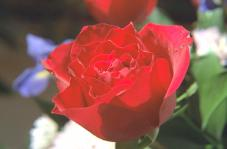
\includegraphics[width=\textwidth]{../SRC/testorig.jpg}
        \caption{Image originale sans message (cover)}
        \label{img:8}
    \end{subfigure}
    ~ %add desired spacing between images, e. g. ~, \quad, \qquad, \hfill etc. 
      %(or a blank line to force the subfigure onto a new line)
    \begin{subfigure}[b]{0.45\textwidth}
        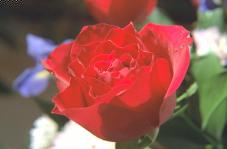
\includegraphics[width=\textwidth]{../SRC/toto.jpg}
        \caption{Image contenant le message (stego)}
        \label{img:9}
    \end{subfigure}
    \caption{Résultats de l'insertion d'un message dans une image}\label{fig:insert}
\end{figure}
Comme nous pouvons le constater grâce à la fonction compare dans l'image \ref{img:10}, nous pouvons distinguer un artefact en haut à gauche dans l'image stego. Cela réside dans le fait que notre message étant relativement court\footnote{Message ici incrusté : \enquote{salut les jean georgios}} et ne modifie alors que les premiers coefficients DCT.
\begin{figure}[H]
    \centering
    
\includegraphics[width=0.5\textwidth]{img/test.jpg}
    \caption{Résultat du compare entre le cover et le stego}
    \label{img:10}
\end{figure}
~\\\par
Afin de récupérer un message présent dans une image stego, nous avons aussi implémenté la fonction suivante :\\
% \begin{lstlisting}[language=C,style=customc]
 Code à faire
% \end{lstlisting}
~\\\par
Cependant, comme nous avons pu le voir, ici l'information n'est pas répartie sur toute l'image ce qui va permettre l'apparition d'un artefact sur l'image. Afin de palier à cela, nous pouvons utiliser un système de clé permettant de diffuser l'information dans toute l'image. Pour cela, nous avons modifié notre fonction $insert\_lsb$ afin que celle-ci demande à l'utilisateur s'il souhaite utiliser une clé.\\
Nous pouvons alors avoir le résultat suivant sur les images testés :
\begin{figure}[H]
    \centering
    \begin{subfigure}[b]{0.45\textwidth}
	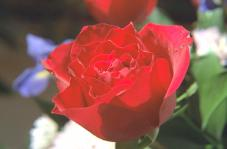
\includegraphics[width=\textwidth]{../SRC/testorig.jpg}
	\caption{Image originale sans message (cover))}
	\label{img:11}
    \end{subfigure}
    ~
    \begin{subfigure}[b]{0.45\textwidth}
	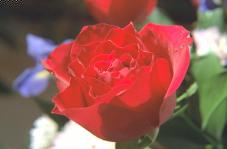
\includegraphics[width=\textwidth]{../SRC/tata.jpg}
	\caption{Image contenant le message (stego) avec clé}
	\label{img:12}
    \end{subfigure}
    \label{fig:key}
\end{figure}
Comme nous pouvons le voir, un artefact est toujours présent en haut à gauche de l'image mais est beaucoup moins important. Si nous réalisons l'opération avec différentes clés, ce dernier change de forme et peut ainsi disparaître.\\\par
Afin de réaliser des histogrammes des coefficients DCT de nos images (et d'ainsi pouvoir comparer la cover image et la stego image), nous avons mis en place la fonction suivante :
\begin{lstlisting}[style=customc]
void get_histo (JPEGimg *img, char* filename)
{
    char* dct_histo[255] = {0};
    FILE *filehisto = fopen(filename, "w");
    int comp, lin, col, pos, i;

    for (comp=0; comp<img->cinfo.num_components; comp++){
	for (lin=0; lin<img->cinfo.comp_info[comp].height_in_blocks; lin++){
	    for (col=0; col<img->cinfo.comp_info[comp].width_in_blocks; col++){
		for (pos=1; pos<64; pos++){
		    dct_histo[img->dctCoeffs[comp][lin][col][pos]+128]++;
		}
	    }
	}
    }

    for (i = 0; i < 255; ++i){
	fprintf(filehisto, "%d\n", dct_histo[i]);
    }
    fclose(filehisto);
}
\end{lstlisting}
Nous pouvons alors retrouver les histogrammes suivants qui nous permettent de comparer les histogrammes d'un cover et d'un stego entre $-15$ et $15$ :
\begin{figure}[H]
    \centering
    \begin{subfigure}[b]{0.45\textwidth}
	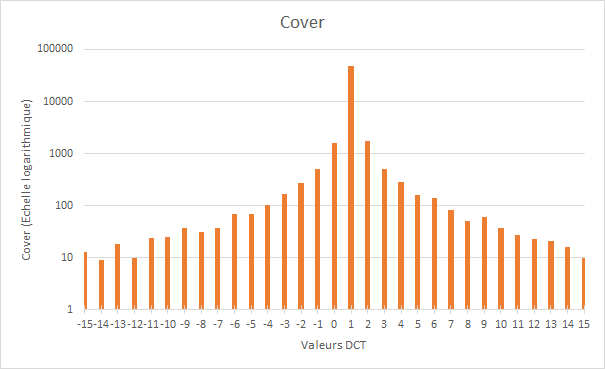
\includegraphics[width=\textwidth]{img/cover_histo.png}
	\caption{Histogramme des DCT du cover}
	\label{img:13}
    \end{subfigure}
    ~
    \begin{subfigure}[b]{0.45\textwidth}
	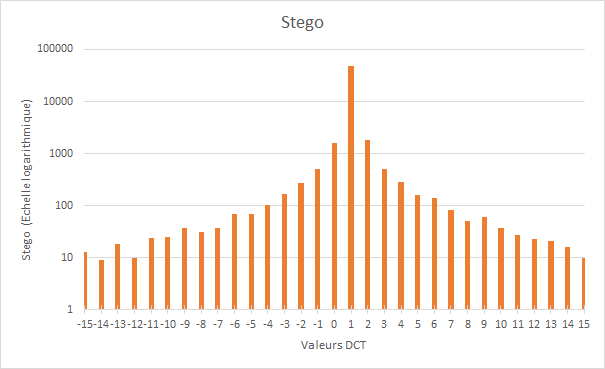
\includegraphics[width=\textwidth]{img/stego_histo.png}
	\caption{Histogramme des DCT du stego}
	\label{img:14}
    \end{subfigure}
    \caption{Histogrammes des coefficients DCT du cover et du stego}\label{fig:histo}
\end{figure}
Si l'on met les deux histogrammes en un seul, nous retrouvons le résultat suivant :
\begin{figure}[H]
    \centering
    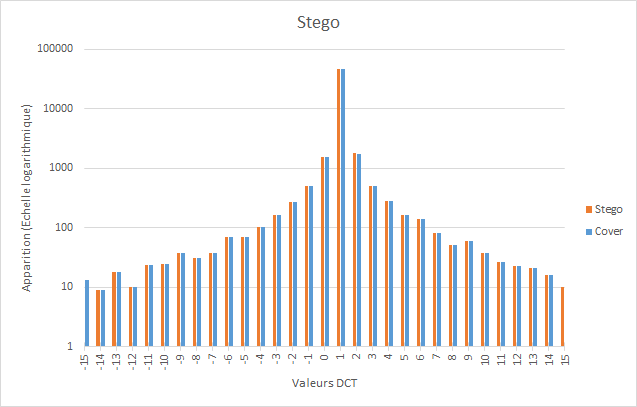
\includegraphics[width=.7\textwidth]{img/both_histo.png}
    \caption{Histogramme combiné du cover et du stego}
    \label{img:15}
\end{figure}
Ainsi on peut remarquer que l'insertion LSB alliée à un système de clé ne va pas beaucoup influencer les coefficients DCT. Ceci est un bon point permettant de n'altérer que subtilement le cover.